% !TEX TS-program = pdflatex
% !TeX program = pdflatex
% !TEX encoding = UTF-8
% !TEX spellcheck = en_US

\documentclass[xcolor=table]{beamer}


%\usepackage{fullpage}
%\usepackage[left=2.8cm,right=2.2cm,top=2 cm,bottom=2 cm]{geometry}
\setbeamersize{text margin left=10pt,text margin right=10pt}



%\usepackage[T1]{fontenc}
\usepackage{textcomp}
\usepackage[utf8]{inputenc}
%\usepackage[french,english]{babel}
\usepackage{arabtex}
\usepackage{txfonts}
\usepackage{tipa}
\usepackage[]{graphicx}
\usepackage{multirow}
\usepackage{hyperref}
\usepackage{colortbl}
\usepackage{tabularray}
\usepackage{listingsutf8}
\usepackage{wrapfig}
\usepackage{multicol}
\usepackage[export]{adjustbox} %for images in table, also for frame
\usepackage[many]{tcolorbox}
\usepackage{wasysym}
\usepackage[lined]{algorithm2e}
\usepackage{alltt} %verbatim with commands
\usepackage{longtable}
\usepackage{tabu}

\usepackage{CJKutf8}

\usepackage{amsmath,amssymb, amsfonts} 

%\usepackage{newtxtext,newtxmath}


%\usepackage{acolor}


\definecolor{lightblue}{HTML}{D0D2FF}
\definecolor{lightyellow}{HTML}{FFFFAA}
\definecolor{darkblue}{HTML}{0000BB}
\definecolor{olivegreen}{HTML}{006600}
\definecolor{darkgreen}{HTML}{008B45} %009B55
\definecolor{violet}{HTML}{6600CC}
\definecolor{deeppink}{HTML}{FF1493}
\definecolor{orangey}{HTML}{FFBB00}


\makeatletter
\def\beamer@calltheme#1#2#3{%
	\def\beamer@themelist{#2}
	\@for\beamer@themename:=\beamer@themelist\do
	{\IfFileExists{\beamer@themelocation/#3\beamer@themename.sty}{%
	\usepackage[{#1}]{\beamer@themelocation/#3\beamer@themename}}{\usepackage[{#1}]{#3\beamer@themename}}
		
	}%
}

\def\usefolder#1{
	\def\beamer@themelocation{#1}
}
\def\beamer@themelocation{}
\makeatother

\usefolder{../../extra/beamer-themes}

\usetheme{Karim} % Antibes Boadilla Warsaw Karim

\beamertemplatenavigationsymbolsempty

\let\oldcite\cite
\renewcommand{\cite}[1]{{\bfseries\color{blue}\oldcite{#1}}}

\tcbuselibrary{listings}


%\renewcommand{\baselinestretch}{1.5}

\def\supit#1{\raisebox{0.8ex}{\small\it #1}\hspace{0.05em}}

\AtBeginSection{%
	\begin{frame}
		\sectionpage
	\end{frame}
}

\newcommand{\rottext}[2]{%
	\rotatebox{90}{%
	\begin{minipage}{#1}%
		\raggedleft#2%
	\end{minipage}%
	}%
}


\institute{ %
Laboratoire de la Communication dans les Systèmes Informatiques (LCSI)
\par
École  nationale Supérieure d'Informatique (ESI), Algiers, Algeria
}
\author[Abdelkrime Aries (2023/2024)] %
{Abdelkrime Aries}
%\titlegraphic{
\includegraphics[height=1cm]{../img/esi-logo.png}%\hspace*{4.75cm}~


\date{Academic year: 2023/2024} %\today

\titlegraphic{%
	
\includegraphics[height=1cm]{../../img/misc/esi-logo.png}%
	\hspace{2cm}%
	
\includegraphics[height=1cm]{../../img/misc/lcsi-logo.png}%
	\hspace{2cm}%
	
\includegraphics[height=1.5cm]{../../img/misc/esi.nlp-logo.png}%
}

%\setbeamertemplate{headline}{}

\newcommand{\kurl}[1]{{\scriptsize\bfseries\color{orangey}\url{#1}}}

\newcommand{\keyword}[1]{\textcolor{red}{\bfseries\itshape #1}}
\newcommand{\expword}[1]{\textcolor{olivegreen}{#1}}
\newcommand{\optword}[1]{\textcolor{violet}{\bfseries #1}}

\makeatletter
\newcommand\mysphere{%
	\parbox[t]{10pt}{\raisebox{0.2pt}{\beamer@usesphere{item projected}{bigsphere}}}}
\makeatother

%\let\oldtabular\tabular
%\let\endoldtabular\endtabular
%\renewenvironment{tabular}{\rowcolors{2}{white}{lightblue}\oldtabular\rowcolor{blue}}{\endoldtabular}


%\NoAutoSpacing %french autospacing after ":"

\def\graphpath{}

\newcommand{\changegraphpath}[1]{\def\graphpath{#1}}


\newcommand{\vgraphpage}[2][.84\textheight]{%
%	\begin{center}%
		\includegraphics[height=#1]{\graphpath #2}%
%	\end{center}%
}

\newcommand{\hgraphpage}[2][\textwidth]{%
%	\begin{center}%
		\includegraphics[width=#1]{\graphpath #2}%
%	\end{center}%
}

\newcommand{\graphpage}[2][]{%
	\includegraphics[#1]{\graphpath #2}%
}

\bibliographystyle{apalike}

\newcommand{\insertbibliography}[2]{
	\appendix
	\section*{Bibliography}
	\nocite{#2}
%	\makeatletter % to change template
%	\setbeamertemplate{headline}[default] % not mandatory, but I though it was better to set it blank
%	\def\beamer@entrycode{\vspace*{-\headheight}} % here is the part we are interested in :)
%	\makeatother
	\begin{multicols*}{2}[\frametitle{\insertsection} \usebeamertemplate*{frametitle}]%\usebeamertemplate*{frametitle}\frametitle{Références}
		\tiny
		\bibliography{#1}
	\end{multicols*}
}

\definecolor{my-grey}{RGB}{233, 233, 233}

\newcommand{\insertlicence}{
	\begin{frame}[plain]
	\frametitle{License: CC-BY 4.0}

	\begin{tcolorbox}[colback=cyan,
		colframe=cyan,  
		arc=0pt,outer arc=0pt,
		valign=top, 
		halign=center,
		width=\textwidth]
		
		
\includegraphics[width=.5cm]{../../img/licence/cc_icon_white_x2.png}
		
\includegraphics[width=.5cm]{../../img/licence/attribution_icon_white_x2.png}
		
		\color{white}
		\bfseries Attribution 4.0 International (CC BY 4.0) \\
		\tiny \url{https://creativecommons.org/licenses/by/4.0/deed.en}
		
	\end{tcolorbox}\vspace{-.5cm}
	\begin{tcolorbox}[colback=my-grey,
		colframe=my-grey,  
		center, arc=0pt,outer arc=0pt,
		valign=top, 
		halign=left,
		width=\textwidth]
		
		\tiny
		
		\begin{center}
			\bfseries\Large
			You are free to:
		\end{center}
		
		\begin{minipage}{0.83\textwidth}
			\begin{itemize}
				\item[] \textbf{Share} — copy and redistribute the material in any medium or format
				\item[] \textbf{Adapt} — remix, transform, and build upon the material
				for any purpose, even commercially.
			\end{itemize}
		
			\vspace{12pt}
		
			\textit{The licensor cannot revoke these freedoms as long as you follow the license terms.}
		\end{minipage}
		\begin{minipage}{0.15\textwidth}
			
\includegraphics[width=\textwidth]{../../img/licence/FreeCulturalWorks_seal_x2.jpg}
		\end{minipage}
	
		
		\begin{center}
			\bfseries\Large
			Under the following terms:
		\end{center}
		
		\begin{itemize}
			\item[] \textbf{Attribution} — You must give appropriate credit, provide a link to the license, and indicate if changes were made. You may do so in any reasonable manner, but not in any way that suggests the licensor endorses you or your use.
			\item[] \textbf{No additional restrictions} — You may not apply legal terms or technological measures that legally restrict others from doing anything the license permits.
		\end{itemize}
		
	\end{tcolorbox}
	
%	\begin{center}
%		\bfseries Attribution 4.0 International (CC BY 4.0)
%		\url{https://creativecommons.org/licenses/by/4.0/deed.fr}
%	\end{center}

%	\tiny
%
%	Vous êtes autorisé à : 
%	\begin{itemize}
%		\item \textbf{Partager} — copier, distribuer et communiquer le matériel par tous moyens et sous tous formats
%		\item \textbf{Adapter} — remixer, transformer et créer à partir du matériel
%	\end{itemize}
%	
%	Selon les conditions suivantes : 
%	\begin{itemize}
%		\item \textbf{Attribution} — Vous devez créditer l'Œuvre, intégrer un lien vers la licence et indiquer si des modifications ont été effectuées à l'Oeuvre. Vous devez indiquer ces informations par tous les moyens raisonnables, sans toutefois suggérer que l'Offrant vous soutient ou soutient la façon dont vous avez utilisé son Oeuvre.
%		\item \textbf{Pas d'Utilisation Commerciale} — Vous n'êtes pas autorisé à faire un usage commercial de cette Oeuvre, tout ou partie du matériel la composant. 
%		\item \textbf{Pas de restrictions complémentaires} — Vous n'êtes pas autorisé à appliquer des conditions légales ou des mesures techniques qui restreindraient légalement autrui à utiliser l'Oeuvre dans les conditions décrites par la licence.
%	\end{itemize}

	\end{frame}
}

\settowidth{\leftmargini}{\usebeamertemplate{itemize item}}
\addtolength{\leftmargini}{\labelsep}

\AtBeginDocument{
	\newcolumntype{L}[2]{>{\vbox to #2\bgroup\vfill\flushleft}p{#1}<{\egroup}} 
	
	\begin{frame}[plain]
		\maketitle
	\end{frame}

	\insertlicence
}


% needs etoolbox; to break links after -
\appto\UrlBreaks{\do\-}


\makeatletter
\newcommand{\xRightarrow}[2][]{\ext@arrow 0359\Rightarrowfill@{#1}{#2}}
\makeatother


\usefonttheme{structurebold}
%\usefonttheme{professionalfonts}


% figure caption
\setlength\abovecaptionskip{2pt}

% equations
\AtBeginDocument{
\abovedisplayskip=0pt
\abovedisplayshortskip=0pt
\belowdisplayskip=0pt
\belowdisplayshortskip=0pt
}


\title[ESI - NLP: 06- Parsing]%
{Natural Language Processing\\Chapter 06\\Parsing} 

\changegraphpath{../img/parsing/}

\begin{document}
	
\begin{frame}
\frametitle{Natural Language Processing}
\framesubtitle{Parsing: Introduction}

\begin{exampleblock}{Example of two sentences}
	\begin{center}
		\Large\bfseries
		The student wrote a solution with a pen. 
		
		The student wrote a solution with an explanation.
	\end{center}
\end{exampleblock}

\begin{itemize}
	\item Who wrote the solution?
	\item What instrument did he use to write?
	\begin{itemize}
		\item A pen? An explanation?
	\end{itemize}
	\item Did the student write something else with the solution?
	\begin{itemize}
		\item A pen? An explanation?
	\end{itemize}
	\item How did you deduce all of this?
\end{itemize}

\end{frame}

\begin{frame}
\frametitle{Natural Language Processing}
\framesubtitle{Parsing: Some humor}

\begin{center}
	\vgraphpage{humor/humor-parse.jpg}
\end{center}

\end{frame}

\begin{frame}
\frametitle{Natural Language Processing}
\framesubtitle{Parsing: Plan}

\begin{multicols}{2}
%	\small
\tableofcontents
\end{multicols}
\end{frame}

%===================================================================================
\section{Syntactic structures}
%===================================================================================

\begin{frame}
\frametitle{Parsing}
\framesubtitle{Syntactic structures}

\begin{itemize}
	\item A sentence can be well formed syntactically but not semantically
	\begin{itemize}
		\item E.g. \expword{Green uncolored ideas sleep furiously.}
	\end{itemize}
	\item Several theories
	\begin{itemize}
		\item Generative grammar
		\item Dependency grammar
		\item Categorical grammar
		\item Stochastic grammars
		\item Functional grammars
	\end{itemize}
	
\end{itemize}

\end{frame}

\subsection{Constituency formalism}

\begin{frame}
\frametitle{Parsing: Syntactic structures}
\framesubtitle{Constituency formalism}

\begin{itemize}
	\item Each word in a sentence has a \keyword{PoS}
	\begin{itemize}
		\item E.g. \expword{The/DT course/NN is/VP interesting/AJ}
	\end{itemize}
	\item One or many words having certain PoS form a \keyword{phrase}
	\begin{itemize}
		\item E.g. \expword{[ The/DT course/NN ]\textsubscript{NP} [ is/VP interesting/AJ ]\textsubscript{VP}}
	\end{itemize}
\end{itemize}

\begin{center}
	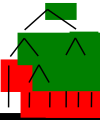
\includegraphics[width=0.3\textwidth]{../img/intro/const_gram.pdf}
\end{center}

\end{frame}

\begin{frame}
\frametitle{Parsing: Syntactic structures}
\framesubtitle{Constituency formalism: Context-free grammars (CFG)}

\begin{minipage}{.68\textwidth}
\begin{itemize}
	\item $G <\Sigma, N, P, S>$ is a grammar.
	\item $\Sigma$ is its vocabulary: set of terminal symbols
	\begin{itemize}
		\item \expword{$\Sigma$ = \{the, little, cat, eats, a, fish, ...\}}
	\end{itemize}
	\item $N$ is the set of variables: set of non terminal symbols 
	\begin{itemize}
		\item \expword{$N$ = \{S, NP, VP, DT, N, AJ, ...\}}
	\end{itemize}
\end{itemize}
\end{minipage}
\begin{minipage}{.3\textwidth}
	\hgraphpage{humor/humor-chomsky.jpg}
\end{minipage}

\begin{itemize}
	\item $S \in N$ is the axiom.
	\item $P$ is the set of production rules.
	\item The rules have the form $A \rightarrow \beta \text{ where } A \in N,\, \beta \in (\Sigma \cup N)^*$
	\begin{itemize}
		\item \expword{S \textrightarrow NP VP}
		\item \expword{NP \textrightarrow DT AJ N \textbar\ DT N}
		\item \expword{VP \textrightarrow V NP}
	\end{itemize}
\end{itemize}

\end{frame}

\begin{frame}
\frametitle{Parsing: Syntactic structures}
\framesubtitle{Constituency formalism: Probabilistic CFG (PCFG)}

\begin{itemize}
	\item \textbf{Problem}: When parsing CFGs, sometimes we find more than one rule to execute.
	\item \textbf{Solution}: Attribute for each rule a probability of occurrence.
	\item Let $G <\Sigma, N, P, S>$ be a grammar.
	\item Rules have the form $A \rightarrow \beta\, [p] \text{ where } A \in N,\, \beta \in (\Sigma \cup N)^*$
	\item $p$ is the rule's occurrence probability
	\item This probability is estimated using an annotated corpus (\keyword{TreeBank})
\end{itemize}

\begin{block}{Rules probability estimation}
	\[
	P(A \rightarrow \beta | A) = \frac{C(A \rightarrow \beta)}{C(A)}
	\]
\end{block}

\end{frame}

\subsection{Dependency formalism}

\begin{frame}
\frametitle{Parsing: Syntactic structures}
\framesubtitle{Dependency formalism}

\begin{itemize}
	\item One or more words fulfill a \keyword{syntactic function}
	\begin{itemize}
		\item Ex. \expword{subject, object, etc.}
	\end{itemize}
	\item Syntactic links between words in a sentence are called: \keyword{dependencies}
	\begin{itemize}
		\item E.g. \expword{The cat eats a fish}: here ``cat" is the \expword{subject} of the verb ``eats"
	\end{itemize}
	\item A dependency relation connects a word called \keyword{syntactic head} with another called \keyword{dependent}
\end{itemize}

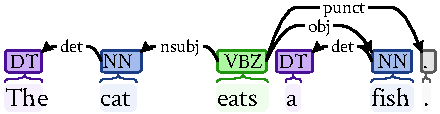
\includegraphics[width=\textwidth]{../img/intro/dep_gram_.pdf}

\end{frame}

\begin{frame}
\frametitle{Parsing: Syntactic structures}
\framesubtitle{Dependency formalism: Dependency relations}

\begin{table}
	\small
	\begin{tblr}{
			colspec = {p{.25\textwidth}p{.35\textwidth}p{.35\textwidth}},
			row{odd} = {lightblue},
			row{even} = {lightyellow},
			row{1} = {darkblue},
			row{6} = {darkblue},
			colsep = 2pt,
			rowsep= 1pt,
		}
		\textcolor{white}{Basic dep.} & \textcolor{white}{Description} & \textcolor{white}{Example}\\
		nsubj & nominal subject & The \underline{people} \textbf{win}\\
		obj & direct object & I \textbf{present} the \underline{course}\\
		iobj & indirect object & He \textbf{send} \underline{me} a mail\\
		csubj & clausal subjects & What she \underline{said} \textbf{makes} sense\\
		
%		\rowcolor{darkblue}
		\textcolor{white}{Nouns dep.} & \textcolor{white}{Description} & \textcolor{white}{Example}\\
		amod & adjectival modifier & The \underline{modest} \textbf{girl}\\
		det & determiner & \underline{The} \textbf{girl}\\
		nmod & nominal modifier & The \underline{result} of the \textbf{race}\\
		nummod & numeric modifier & I ate \underline{3} \textbf{candies}\\
		
	\end{tblr}

	\vskip8pt\caption{Some Stanford universal dependency relations \cite{2014-de-marneffe-al} (\url{https://universaldependencies.org/u/dep/index.html})}
\end{table}

\end{frame}

%===================================================================================
\section{Constituency parsing}
%===================================================================================

\begin{frame}
\frametitle{Parsing}
\framesubtitle{Constituency parsing}

\begin{itemize}
	\item Context-Free grammar (CFG): The most used formal system to model constituency structure
	\item Parsing 
	\begin{itemize}
		\item \optword{ascending}: We attribute a PoS to each word in the sentence. Then, we search for phrases which generates a combination of PoS and phrases. We do this until we get the axiom \keyword{S}
		\item \optword{descending}: from \keyword{S}, we search for the rules that generate the sentence. We use words to guide the selection of rules.
	\end{itemize}
\end{itemize}

\begin{center}
	\begin{tabular}{|p{.25\textwidth}|p{.3\textwidth}|p{.3\textwidth}|}
	\hline
	& Classical & Statistical \\
	\hline
	Ascending & \optword{CKY}, LR & \optword{probabilistic CKY}\\
	\hline
	Descending & Early, LL, Recursive descent & \\
	\hline
\end{tabular}
\end{center}

\end{frame}

\subsection{CKY algorithm}

\begin{frame}
\frametitle{Parsing: Constituency parsing}
\framesubtitle{CKY algorithm}

\begin{itemize}
	\item \keyword{Cocke-Kasami-Younger} algorithm
	\item Bottom-up analysis (Ascending)
	\item Prerequisites: Chomsky normal form (CNF)
\end{itemize}

\begin{minipage}{.4\textwidth}
	\begin{definition}[CNF]
		\[G <\Sigma, N, P, S>\]
		\[A \rightarrow  B C \text{ where } A, B, C \in N\]
		\[A \rightarrow w \text{ where } w \in \Sigma\]
	\end{definition}
\end{minipage}
\begin{minipage}{.56\textwidth}
	\begin{block}{CNF building}
	\tiny
	\begin{algorithm}[H]
		\KwData{A proper grammar $G <\Sigma, N, P, S>$}
		\KwResult{CNF grammar $G' <\Sigma, N', P', S>$}
		
		Replace all terminals $\sigma$ in each rule's right hand side by a variable $v$\;
		Add the rule $v \rightarrow\ \sigma$ to $N'$\;
		\ForEach{rule $A \rightarrow\  \alpha $}{
			\If{$\alpha$ has more than 2 variables}{
				Keep the first variable and create a new rule\;
				The new variable generates the rest of variables\;
				Redo the same thing till all rules are CNF\;
			}
		}
	\end{algorithm}
	\end{block}
\end{minipage}

\end{frame}

\begin{frame}
\frametitle{Parsing: Constituency parsing}
\framesubtitle{CKY algorithm: Sentence Recognition}

\begin{block}{CKY: Sentence Recognition}
	\scriptsize\vspace{-3pt}
	\begin{algorithm}[H]
		\KwData{A grammar $G <\Sigma, N, P, S>$ in CNF; a sentence $w = w_1 \ldots w_n$}
		\KwResult{$T[n, n]$}
		
		\lFor{$ i = 1 \ldots n$}{ %\tcc*{Initialiser le diagonal}
			$T[i, i] \leftarrow \{ (A, 0, 0, 0) / (A \rightarrow w_i) \in P \} $
		}
		
		\For{$ i = (n-1) \ldots 1$ }{
			\For{$ j = (i+1) \ldots n $}{
				\For{$ k = i \ldots (j-1) $}{
					\ForEach{$A$ such as $(A \rightarrow B C) \in P $ and $B \in T[i, k]$ et $C \in T[k+1, j]$}{
						$iB \leftarrow index(B, T[i, k])$ ;
						$iC \leftarrow index(C, T[k+1, j])$ \;
						$T[i, j] \leftarrow T[i, j] \cup \{(A, k, iB, iC)\}$ \;
					}
				}
			}
		}
		
		\lIf{$``S" \notin T[1, n] $} {
			Error ``The sentence was not recognized"
		}
		\vspace{-3pt}
	\end{algorithm}
\end{block}

\end{frame}

\begin{frame}
\frametitle{Parsing: Constituency parsing}
\framesubtitle{CKY algorithm: Tree Building}

\begin{block}{CKY: Tree Building}
	\scriptsize\vspace{-3pt}
	\begin{algorithm}[H]
		\SetKwFunction{FConst}{build}
		\SetKwProg{Fn}{function}{}{end}
		
		\KwData{$T[n, n]$}
		\KwResult{parse tree's root: $r \leftarrow \varnothing$}
		
		\If{$``S" \in T[1, n] $} {
			$r \leftarrow $ \FConst{$1, n, index(``S", T[1, n])$}\;
		}
		
		\Fn{\FConst{$i, j, pos$}}{
			$ (A, k, iB, iC) \leftarrow T[i, j][pos] $\;
			n $\leftarrow$ new Node()\;
			n.value $\leftarrow  A$ \;
			\If{$k>0$}{
				n.left $\leftarrow$ \FConst{$i, k, iB$}\;
				n.right $\leftarrow$ \FConst{$k+1, j, iC$}\;
			}
			\Return n\;
		}		
%		\vspace{-3pt}
	\end{algorithm}
\end{block}

\end{frame}

\begin{frame}
\frametitle{Parsing: Constituency parsing}
\framesubtitle{CKY algorithm: Exercise}

\begin{exampleblock}{Example of a grammar}
	\begin{itemize}
		\item S \textrightarrow\ NP VP \textbar\ VP
		\item VP \textrightarrow VB NP
		\item NP \textrightarrow\ DT AJ NN \textbar\ DT NN \textbar\ PR 
		\item PR \textrightarrow\ he \textbar\ she \textbar\ they \textbar\ you
		\item VB \textrightarrow\ form \textbar\ forms \textbar\ eats \textbar\ fish
		\item DT \textrightarrow\ a \textbar\ the
		\item AJ \textrightarrow\ little \textbar\ big \textbar\ red 
		\item NN \textrightarrow\ form \textbar\ forms \textbar\ cat \textbar\ fish
	\end{itemize}
\end{exampleblock}\vspace{-6pt}

\begin{itemize}
	\item Analyze the sentence \expword{the fish form a little form} using CKY 
	\item Analyze the sentence \expword{the cat eats a little fish} using CKY
\end{itemize}

\end{frame}

\begin{frame}
\frametitle{Parsing: Constituency parsing}
\framesubtitle{CKY algorithm: Notes}

\begin{minipage}{.53\textwidth}
\begin{itemize}
	\item The result is a binary parse tree. 
	However, in reality, the tree must follow the original grammar designed by syntacticians.
	\begin{itemize}
		\item Add a post-processing step to recover the original tree.
		\item Leave unit productions and modify CKY algorithm in order to accept them.
	\end{itemize}
	\item Syntactic ambiguity problem
	\begin{itemize}
		\item E.g. \expword{I eat rice with a fork.} and \expword{I eat rice with meat.}
%		\item 
	\end{itemize}
\end{itemize}
\end{minipage}
\begin{minipage}{.45\textwidth}
	\hgraphpage{humor/humor-ambiguity.jpg}
\end{minipage}

\end{frame}

\subsection{Probabilistic CKY algorithm}

\begin{frame}
\frametitle{Parsing: Constituency parsing}
\framesubtitle{Probabilistic CKY algorithm}

\begin{itemize}
	\item $G<\Sigma, N, P, S>$ is probabilistic grammar.
	\item The new rules created by transformation into FNC have a probability equal to $1$
	\item $w = w_1 \ldots w_n$ is a sentence to be parsed
	\item $P(T, w) = \prod\limits_{(A_i \rightarrow \beta_i) \in T} P(A_i \rightarrow \beta_i)$ is the probability of a parse tree $T$ given a sentence $w$
	\item $\hat{T}(w) = \arg\max\limits_{T(w)} P(T, w) $ is the most adequate syntactic tree to analyze the sentence $w$
\end{itemize}

\end{frame}

\begin{frame}
\frametitle{Parsing: Constituency parsing}
\framesubtitle{Probabilistic CKY algorithm: Sentence Recognition}

\begin{block}{Probabilistic CKY: Sentence Recognition}
	\scriptsize\vspace{-3pt}
	\begin{algorithm}[H]
		\KwData{A grammar $G <\Sigma, N, P, S>$ in FNC; a sentence $w = w_1 \ldots w_n$}
		\KwResult{$T[n, n, |N|]$}
		
		\lFor{$ i = 1 \ldots n$}{ %\tcc*{Initialiser le diagonal}
			$T[i, i, A] \leftarrow \{ (P(A \rightarrow w_i), 0, A, A) / (A \rightarrow w_i) \in P \} $
		}
		
		\For{$ i = (n-1) \ldots 1$ }{
			\For{$ j = (i+1) \ldots n $}{
				\For{$ k = i \ldots (j-1) $}{
					\ForEach{$A$ such as $(A \rightarrow B C) \in P $ et $T[i, k, B] > 0$ et $T[k+1, j, C] > 0$}{
						$p \leftarrow P(A \rightarrow B C) * T[i, k, B][1] * T[k+1, j, C][1]$\;
						\If{$p > T[i, j, A][1]$}{
							$T[i, j, A] \leftarrow (p, k, B, C)$ \;
						}
					}
				}
			}
		}
		
		\lIf{$T[1, n, S] = 0 $} {
			Error ``The sentence was not recognized"
		}
		\vspace{-3pt}
	\end{algorithm}
\end{block}

\end{frame}


%===================================================================================
\section{Dependency parsing}
%===================================================================================

\begin{frame}
\frametitle{Parsing}
\framesubtitle{Dependency parsing}

\begin{minipage}{.6\textwidth}
\begin{itemize}
	\item \optword{Transition-based parsing} 
	\begin{itemize}
		\item \textbf{Configuration}:  $C = (\sigma, \beta, A)$ where $\sigma$ is a stack, $\beta$ is an input buffer and $A$ is the list of created arcs
		\item $C_{initiale} = ([ROOT], w, \emptyset)$
		\item $C_{finale} = ([ROOT], \varnothing, A)$
%		\item Un ensemble d'actions possibles
	\end{itemize}
\end{itemize}
\end{minipage}
\begin{minipage}{.38\textwidth}
	\hgraphpage{transitions.pdf}
\end{minipage}

%
\vfill

\begin{minipage}{.6\textwidth}
	\begin{itemize}
		\item \optword{Graph-based parsing}
		\begin{itemize}
			\item \textbf{Graph}: $G = (V, E)$ where $V$ is a set of nodes (words) and $E$ is a set of arcs (dependency relations)
			\item \textbf{Results}: $T = (V, F)$ is a sub-graph of $G$ which represents dependency relations
		\end{itemize}
	\end{itemize}
\end{minipage}
\begin{minipage}{.38\textwidth}
	\hgraphpage{graph.pdf}
\end{minipage}

\end{frame}

\subsection{Transition-based}

\begin{frame}
\frametitle{Parsing: Dependency parsing}
\framesubtitle{Transition-based}

\begin{minipage}{.6\textwidth}
	\begin{itemize}
		\item \textbf{Configuration}:  $C = (\sigma, \beta, A)$
		\begin{itemize}
			\item $\sigma$ is a stack
			\item $\beta$ is the input buffer
			\item $A$ is the list of created arcs
			\item $C_{initiale} = ([ROOT], w, \emptyset)$
			\item $C_{finale} = ([ROOT], \varnothing, A)$
		\end{itemize}
	\end{itemize}
\end{minipage}
\begin{minipage}{.38\textwidth}
	\hgraphpage{transitions.pdf}
\end{minipage}

\begin{itemize}
	\item \textbf{Transition}; change from one state to another using actions on:
	\begin{itemize}
		\item $\sigma$: push or pop a word;
		\item $\beta$: remove a word or add one at the beginning;
		\item $A$: add a dependency between 2 words.
	\end{itemize}
	\item \textbf{Oracle}: a trained model to decide the next transition.
\end{itemize}

\end{frame}

\begin{frame}
\frametitle{Parsing: Dependency parsing}
\framesubtitle{Transition-based: Parsing algorithm}

\begin{itemize}
	\item ``$Oracle$" model choose a transition ``$t$"
	\item The function ``$Apply$" execute ``$t$" on the configuration
\end{itemize}

\begin{block}{Dependency parsing using Transitions}
	\begin{algorithm}[H]
		\KwData{The sentence to be parsed: $w= w_1 w_2 \ldots w_n$}
		\KwResult{Dependencies list: $A$}
		
		$C \leftarrow (\sigma=[ROOT], \beta = w, A = \emptyset)$\;
		
		
		\While{$\sigma \ne [ROOT]$ OR $\beta \ne \varnothing$}{
			$t \leftarrow Oracle(C)$\;
			$C \leftarrow Apply(C, t)$\;
		}
	
		\Return $A$ \;
	\end{algorithm}
\end{block}

\end{frame}

\begin{frame}
\frametitle{Parsing: Dependency parsing}
\framesubtitle{Transition-based: Oracle model (training)}

\begin{itemize}
	\item ``Oracle" model learns to infer the transition $\hat{t}$ given:
	\begin{itemize}
		\item current configuration: $ C = (\sigma, \beta, A) $;
		\item possible transitions set $T$;
		\item a function $\Psi$ which calculate a score using some features based on the configuration;
		\item an annotated text (TreeBank).
	\end{itemize}
	\[ \hat{t} = \arg\max\limits_{t \in T} \Psi (t, C, w; \theta) \]

	\item The annotated text must be transformed to a sequence of transactions.
	\item To train ``Oracle" model, the parsing algorithm is used.
	\item The function $\Psi$  can be MaxEnt (the most used), SVM or neural networks.
\end{itemize}

\end{frame}

\begin{frame}
\frametitle{Parsing: Dependency parsing}
\framesubtitle{Transition-based: Oracle model (features)}

\begin{itemize}
	\item \textbf{Stack $\sigma$}:
	\begin{itemize}
		\item The top of the stack;
		\item Its (The top of the stack) PoS.
	\end{itemize}

	\item \textbf{Input buffer $\beta$}:
	\begin{itemize}
		\item The first three words;
		\item Their PoS.
	\end{itemize}

	\item \textbf{Dependencies list $A$}:
	\begin{itemize}
		\item The dependencies that have been estimated.
	\end{itemize}

	\item \textbf{The sentence $w$}:
	\begin{itemize}
		\item The distance between the word in the top of the stack and the first word on the buffer (number of words between them in the sentence $w$).
	\end{itemize}

\end{itemize}

\end{frame}

\begin{frame}
\frametitle{Parsing: Dependency parsing}
\framesubtitle{Transition-based: Arc-standard (possible transitions)}

\begin{itemize}
	\item \optword{SHIFT}: Move the first item in the buffer to the stack
	\[ (\sigma, w_i|\beta, A) \Rightarrow  (\sigma|w_i, \beta, A) \]
	
	\item \optword{ARC-LEFT}: Establish an arc from the first element in the buffer to the top of the stack
	\[ (\sigma|w_i, w_j|\beta, A) \Rightarrow  (\sigma, w_j|\beta, A \cup \{w_j \rightarrow w_i \}) \] 
	
	\item \optword{ARC-RIGHT}: Establish an arc from the top of the stack to the first element in the buffer
	\[ (\sigma|w_i, w_j|\beta, A) \Rightarrow  (\sigma, w_i|\beta, A \cup \{w_i \rightarrow w_j \}) \] 
\end{itemize}

\end{frame}


\begin{frame}
\frametitle{Parsing: Dependency parsing}
\framesubtitle{Transition-based: Arc-standard (example)}

\begin{exampleblock}{Example of unlabeled derivations of the sentence ``He writes the solution and its explanation" using Arc-standard}
	\centering\bfseries\fontsize{5.5}{10}\selectfont
	\begin{tblr}{
			colspec = {llll},
			row{odd} = {lightblue},
			row{even} = {lightyellow},
			row{1} = {darkblue},
			rowsep=0pt,
			colsep=2pt,
		}
		\textcolor{white}{nb. $\sigma$ (stack)} & \textcolor{white}{$\beta$ (input buffer)} & \textcolor{white}{Action} & \textcolor{white}{Added Arc to A} \\
%		\hline
		01. [\textcolor{red}{ROOT}] & \textcolor{red}{He} writes the solution and its explanation & SHIFT & / \\
		02. [ROOT, \textcolor{red}{He}] & \textcolor{red}{writes} the solution and its explanation & ARC-LEFT & He \textleftarrow\ writes\\
		03. [\textcolor{red}{ROOT}] & \textcolor{red}{writes} the solution and its explanation & SHIFT & / \\
		04. [ROOT, \textcolor{red}{writes}] & \textcolor{red}{the} solution and its explanation & SHIFT & / \\
		05. [ROOT, writes, \textcolor{red}{the}] & \textcolor{red}{solution} and its explanation & SHIFT & / \\
		06. [ROOT, writes, the, \textcolor{red}{solution}] & \textcolor{red}{and} its explanation & SHIFT & / \\
		07. [ROOT, writes, the, solution, \textcolor{red}{and}] & \textcolor{red}{its} explanation & SHIFT & / \\
		08. [ROOT, writes, the, solution, and, \textcolor{red}{its}] & \textcolor{red}{explanation} & ARC-LEFT & its \textleftarrow\ explanation\\
		09. [ROOT, writes, the, solution, \textcolor{red}{and}] & \textcolor{red}{explanation} & ARC-LEFT & and \textleftarrow\ explanation\\
		10. [ROOT, writes, the, \textcolor{red}{solution}] & \textcolor{red}{explanation} & ARC-RIGHT & solution \textrightarrow\ explanation\\
		11. [ROOT, writes, \textcolor{red}{the}] & \textcolor{red}{solution} & ARC-LEFT & the \textleftarrow\ solution\\
		12. [ROOT, \textcolor{red}{writes}] & \textcolor{red}{solution} & ARC-RIGHT & writes \textrightarrow\ solution\\
		13. [\textcolor{red}{ROOT}] & \textcolor{red}{writes} & ARC-RIGHT & ROOT \textrightarrow\ writes\\
		14. [ROOT] & $\emptyset$ & END & / \\
%		\hline\hline
	\end{tblr}
\end{exampleblock}

\end{frame}


\begin{frame}
\frametitle{Parsing: Dependency parsing}
\framesubtitle{Transition-based: Arc-eager (possible transitions)}

\begin{itemize}
	\item \optword{SHIFT}: the same as ``Arc-standard"
	
	\item \optword{ARC-LEFT}: Establish an arc from the first element in the buffer to the top of the stack
	\[ (\sigma|w_i, w_j|\beta, A) \xRightarrow{\forall w_k (w_k \rightarrow w_i) \notin A}  (\sigma, w_j|\beta, A \cup \{w_j \rightarrow w_i \}) \] 
	
	\item \optword{ARC-RIGHT}: Establish an arc from the top of the stack to the first element in the buffer
	\[ (\sigma|w_i, w_j|\beta, A) \Rightarrow  (\sigma|w_i w_j, \beta, A \cup \{w_i \rightarrow w_j \}) \] 
	
	\item \optword{REDUCE}: Pop a word if it already has a parent
	\[ (\sigma|w_i, \beta, A) \xRightarrow{\exists w_k (w_k \rightarrow w_i) \in A} (\sigma, \beta, A) \] 
%	\[ (\sigma|w_i, \beta, \mathcal{A}) \overset{\exists w_k (w_k \rightarrow w_i) \in \mathcal{A}}{\Longrightarrow} (\sigma, \beta, \mathcal{A}) \] 
\end{itemize}

\end{frame}

\begin{frame}
\frametitle{Parsing: Dependency parsing}
\framesubtitle{Transition-based: Arc-eager (example)}

\begin{exampleblock}{Example of unlabeled derivations of the sentence ``He writes the solution and its explanation" using Arc-eager}
	\centering\bfseries\fontsize{6}{10}\selectfont
	\begin{tblr}{
			colspec = {llll},
			row{odd} = {lightblue},
			row{even} = {lightyellow},
			row{1} = {darkblue},
			rowsep=0pt,
			colsep=2pt,
		}
%		nb. $\sigma$ (pile) & $\beta$ (tampon) & Action & Arc ajouté à A \\
		\textcolor{white}{nb. $\sigma$ (stack)} & \textcolor{white}{$\beta$ (input buffer)} & \textcolor{white}{Action} & \textcolor{white}{Added Arc to A} \\
%		\hline
		01. [\textcolor{red}{ROOT}] & \textcolor{red}{He} writes the solution and its explanation & SHIFT & / \\
		02. [ROOT, \textcolor{red}{He}] & \textcolor{red}{writes} the solution and its explanation & ARC-LEFT & He \textleftarrow\ writes\\
		03. [\textcolor{red}{ROOT}] & \textcolor{red}{writes} the solution and its explanation & ARC-RIGHT & ROOT \textrightarrow\ writes\\	
		04. [ROOT, \textcolor{red}{writes}] & \textcolor{red}{the} solution and its explanation & SHIFT & / \\	
		05. [ROOT, writes, \textcolor{red}{the}] & \textcolor{red}{solution} and its explanation & ARC-LEFT & the \textleftarrow\ solution \\
		06. [ROOT, \textcolor{red}{writes}] & \textcolor{red}{solution} and its explanation & ARC-RIGHT & writes \textrightarrow\ solution \\
		07. [ROOT, writes, \textcolor{red}{solution}] & \textcolor{red}{and} its explanation & SHIFT & / \\
		08. [ROOT, writes, solution, \textcolor{red}{and}] & \textcolor{red}{its} explanation & SHIFT & / \\
		09. [ROOT, writes, solution, and, \textcolor{red}{its}] & \textcolor{red}{explanation} & ARC-LEFT & its \textleftarrow\ explanation \\
		10. [ROOT, writes, solution, \textcolor{red}{and}] & \textcolor{red}{explanation} & ARC-LEFT & and \textleftarrow\ explanation\\	
		11. [ROOT, writes, \textcolor{red}{solution}] & \textcolor{red}{explanation} & REDUCE & /\\
		12. [ROOT, \textcolor{red}{writes}] & \textcolor{red}{solution} & ARC-RIGHT & writes \textrightarrow\ solution\\
		13. [ROOT, \textcolor{red}{solution}] & $\emptyset$ & REDUCE & / \\
		14. [ROOT] & $\emptyset$ & END & / \\
%		\hline\hline
	\end{tblr}
\end{exampleblock}

\end{frame}

\subsection{Graph-based}

\begin{frame}
\frametitle{Parsing: Dependency parsing}
\framesubtitle{Graph-based}

\begin{minipage}{.6\textwidth}
	\begin{itemize}
		\item Graph-based parsing
		\begin{itemize}
			\item \textbf{Graph}: $G = (V, E)$ where $V$ is the set of nodes (words) and $E$ the set of arcs (dependency relations)
			\item \textbf{Results}: $T = (V, F)$ is a sub-graph of $G$ which represents dependency relations
		\end{itemize}
	\end{itemize}
\end{minipage}
\begin{minipage}{.38\textwidth}
	\hgraphpage{graph.pdf}
\end{minipage}

\begin{itemize}
	\item $\Psi$ is a scoring function, $ \mathcal{T}(G) $ is the set of possible dependency tree over $G$
	\[ \hat{T} = \arg\max\limits_{T \in \mathcal{T}(G)} \Psi(T, w; \theta) \]
	\item This score is calculated based on the score of each arc $\psi$
	\[ \Psi(T, w; \theta) = \sum_{e \in F / T = (V, F)} \psi(e, w; \theta) \]
\end{itemize}

\end{frame}

\begin{frame}
\frametitle{Parsing: Dependency parsing}
\framesubtitle{Graph-based: scoring and training}

\begin{itemize}
	\item Arcs scores depend on some features ($K$ features)
	\[ \psi(e, w; \theta) = \sum_{k = 1}^{K} \theta_k f_k(e, w)  \]
	
	\item Some features
	\begin{itemize}
		\item The stack head, its PoS, its lemma, its prefixes and suffixes
		\item Arc direction
		\item Distance between the head and the dependent
		\item \ldots
	\end{itemize}
	
\end{itemize}

\end{frame}

\begin{frame}
\frametitle{Parsing: Dependency parsing}
\framesubtitle{Graph-based: Chu-Liu/Edmonds parsing}

\begin{itemize}
	\item A new node (ROOT) is created, which has arcs to all existing nodes 
	\item Arcs are weighted where the weight of an arc $e$ is denoted by $G.p(e)$
	\item A \keyword{maximum spanning tree} is constructed from $G$
	\item \keyword{maximum spanning tree}: A maximal acyclic subgraph where all nodes are connected and there is no more than one arc entering to a node
	\item \optword{Contract}: a function that merges two nodes $u$ and $v$ making a cycle $C$
	\begin{itemize}
		\item $\forall e = (u', v) \in E : G.p(e) \leftarrow G.p(e) - G.p((u, v)) $
		\item $\forall e = (v', u) \in E : G.p(e) \leftarrow G.p(e) - G.p((v, u)) $
	\end{itemize}
	\item \optword{Extend}: a function that splits the two nodes $u$ and $v$ of a cycle $C$. The arc that violates the condition ``\textit{no more than one entering arc}" is deleted
\end{itemize}
 
\end{frame}

\begin{frame}
\frametitle{Parsing: Dependency parsing}
\framesubtitle{Graph-based: Chu-Liu/Edmonds parsing (algorithm)}


\begin{block}{Chu-Liu-Edmonds parsing: Maximum spanning tree}
	\scriptsize\vspace{-3pt}
	\begin{algorithm}[H]
		\KwData{a weighted graph $G = (V, E)$, $ ROOT $}
		\KwResult{a spanning tree $T = (V, F)$}
		
		\SetKwFunction{MST}{MaxSpanTree}
		\SetKwProg{Fn}{function}{}{end} 
		
		\Fn{\MST{$G, ROOT$}}{
		
		$F \leftarrow \emptyset$\;
		
		\ForEach{$ v \in V$}{ 
			$bestInArc \leftarrow \arg\max_{e = (u, v) \in E} G.p(e) $;
			$F \leftarrow F \cup meilleurInArc$\;
			\lForEach{$e = (u, v) \in E$}{ 
				$ G.p(e) \leftarrow G.p(e) - G.p(bestInArc) $
			}
			\If{$T = (V, F)$ is not a spanning tree}{
				$C \leftarrow$ a cycle of $F$;
				$G' \leftarrow Contract(G, C)$\;
				$T' \leftarrow MaxSpanTree(G', ROOT)$;
				$T \leftarrow Extend(T', C)$\;
			}
			\Return $T$ \;
		}
	
		}
	\end{algorithm}
\end{block}

\end{frame}

\begin{frame}
\frametitle{Parsing: Dependency parsing}
\framesubtitle{Graph-based: Chu-Liu/Edmonds parsing (Exercise)}

\begin{figure}
	\centering
	\hgraphpage[.8\textwidth]{exp-graph.pdf}
	\caption{Graph of the sentence ``Read the course" }
\end{figure}

\end{frame}


\insertbibliography{NLP06}{*}

\end{document}

